\chapter{Promoting Unselfish Routes}
Traffic congestion has been a perennial problem in many highly urbanized cities across the globe. As government stakeholders tackle this issue by implementing policies and building infrastructure, they are also becoming aware that there is a greater need to promote sustainable driving behaviors among its citizen drivers to fully achieve their goals\cite{Attard2016TheSystems,darnton2008gsr}. It would take long term transformations on the route choice behavior of everyday drivers.

Navigation applications have a great potential in helping cities manage traffic flow at the onset of a traffic congestion. Drivers who commute daily to and from their work, school or business can be distributed and guided to a number of alternative routes with the goal of preventing traffic jams. If the road network is already experiencing traffic congestion on some of its roads, drivers can be directed to less used roads. And crucial to this is the timely delivery of navigational information that will aid the driver in their decision making. 

There are a number of factors that affect individual route choice \cite{Ben-Elia2015ResponseReview,Chorus2006TravelReview}. Arguably, the most important factor is travel time and we see this information constantly highlighted whenever we search for driving directions in most modern applications. While this is especially true in urgent circumstances, we found in Chapter 4 that in most cases, road and route familiarity and their closeness to what drivers use regularly play a bigger role in the decision making process. For these reasons, it can be a challenge if we suggest unselfish routes to daily commuters. Unlike optimal routes that are recommended because they have the fastest travel time or shortest distance, unselfish routes are alternatives that are typically sub-optimal (slower or longer). So now the question is if it would be possible to convince drivers to choose a sub-optimal unselfish route over an optimal one. In this chapter, I explore the effects of adding motivative and familiarity navigational information to route recommendations. I discuss the results of an online experiment in a within-subject design with 28 participants. Participants were asked to choose between an optimal and an unselfish route for 28 times under different conditions. In this chapter, I:
\begin{itemize}
    \item describe the concept of adding combinations of motivative and familiarity information to route recommendations;
    \item discuss how different combinations affect individual route choice;
    \item discuss how their individual route choice were correlated with their General Causality Orientation and Motivation to Volunteer scores; and
    \item discuss design implications for presenting recommendations that promotes unselfish routes.
\end{itemize}

\section{Navigation Apps as Civic Technology}
If future navigation applications will become tools to aid government stakeholders and urban planners in accomplishing their traffic management and sustainability goals, we have to start designing technical solutions from the point of view of civic technologies. By definition, civic technologies are tools that facilitate the collaboration between governments and their citizens for the public good\cite{Mandarano2010Civic}. In future traffic management systems, it would require a great amount of effort from governments to establish communication and technology platforms that will allow long term behavioral transformation among its citizens. On the part of the citizens, they have to be motivated enough in order to sustain or even be convinced that they should adopt or participate in such prosocial behavior. 

In our envisioned future, cities must collectively work together towards the common goal of avoiding traffic congestion. A more sustainable future is when citizens will voluntarily change their driving behaviors and daily routes because they are increasingly aware of its benefits for them and others.

Civic technologies have been used to organize citizens or small communities towards common goals. And in order for them to achieve tangible outcomes, citizens are usually asked to volunteer their time and effort for a number of reasons, most of the time without monetary incentives. Thus, despite effectively communicating lofty goals of achieving social good, designers of civic technologies still face the challenge of encouraging citizens to contribute and continue participation. 

\section{Self-Determination Theory}
Motivation is the primary driving force in starting and performing any work, learning or task. These are often categorized as intrinsic and extrinsic motivation, wherein the former was proven to have positive effects on work performance\cite{gagne2005self}. One established theory on motivation, The Self-Determination Theory (SDT)\cite{ryan2000intrinsic}, expands this categorization by introducing a spectrum of extrinsic motivation. Originally, theories focus on the task as the origin of motivation. In SDT, we are given a framework to understand how people who perform the task and their internalization of its reasons and goals affect motivation. Thus, motivation is a product of the interaction between the task, the person, and their environment.

In SDT's framework, there are three types of motivation: intrinsic motivation, extrinsic motivation and amotivation. And when \textit{``an individual acquires an attitude, belief, or behavioral regulation and progressively transforms it into a personal value, goal, or organization,''}\cite{ryan2000intrinsic} these get internalized into autonomous and controlled motivation, or lack of motivation. 

In designing civic technologies, it is ideal that we engage citizens with causality orientations and behavioral regulation styles that facilitate autonomous motivation. SDT's framework describes a set of general causality orientations that describe ways people orient themselves across different environments and regulate their behavior (Table \ref{tab:gcos}. 

\begin{table}[h]
    \caption{The general causality orientations according to the Self-Determination Theory framework.}
	\label{tab:gcos}
	\centering
	\begin{tabular}{l l}
	    \hline\hline
		\textbf{Autonomy orientation} & Oriented towards environments that stimulate intrinsic \\
        & motivation, are optimally challenging, provide \\
        & informational feedback, and allow choice. Tends to \\
        & display greater self-initiation, seek activities that \\
        & are interesting and challenging, and take greater responsibility \\
        & for his or her own behavior. \\
        \textbf{Controlled orientation} & Oriented toward being controlled by rewards, deadlines, \\
        & structures, ego involvements, and the directives of others. \\
        & Likely to be dependent on rewards or other controls, and may \\
        & be more attuned to what others demand than to what they want \\
        & for themselves \\
        \textbf{Impersonal orientation} & Believes that attaining desired outcomes is beyond his or her \\
        & control and that achievement is largely a matter of luck \\
        & or fate. Likely to be anxious and feel very ineffective. \\
        & Has no sense of being able to affect outcomes or cope \\ 
        & with demands or changes. Tends to be amotivated and to want \\
        & things to be as they always were. \\
		\hline
	\end{tabular}
\end{table}

Regardless of the causality orientation, human behavior can be regulated and processed in a number ways. This resulted to a spectra of extrinsic motivation, namely \textit{external regulation} (most externally processed), \textit{introjection}, \textit{identification}, and \textit{integration} (most internally processed). If a person has a \textit{identification} or \textit{integration} regulatory style, and autonomy oriented, they are predicted to internalize \textit{autonomous motivation}. On the other hand, a person needs to be \textit{externally regulated} or has \textit{introjection} regulatory style, and control oriented, they are predicted to internalize \textit{controlled motivation}. 

To achieve that, SDT also claims that the environment within which a person performs a task must support three basic psychological needs that are universal: autonomy, control and relatedness. Thus, we must aim to design future navigation applications as autonomy-supportive environments in order to support driver's instructed actions and adoption of unselfish route choices.

\section{Motivative Information}
In order to promote the use of unselfish routes without any explicit messaging diversification and incentive structures, we hypothesize that the simple addition of relevant navigational information must support the three psychological needs (autonomy, competence, relatedness) and an autonomous orientation. Specifically, we propose to include three types of motivative information as shown in Table \ref{tab:motive-info}. 

\begin{table}[h]
    \caption{The types of motivative information.}
	\label{tab:motive-info}
	\centering
	\begin{tabular}{l l}
	    \hline\hline
		\textbf{Motivative Information} & \textbf{Template} \\
		\hline
		\textbf{Critical mass} & \textbf{Optimal} \\
		& 70 drivers are following this now. \\
		& \textbf{Unselfish} \\
		& 30 drivers are following this now. \\
        \textbf{Valence framing} & \textbf{Optimal} \\
        & Avg Travel Time of everyone can be 0 min faster \\
		& \textbf{Unselfish} \\
		& Avg Travel Time of everyone can be <N> min faster \\
        \textbf{Simple positive framing} & \textbf{Optimal} \\
        & Fastest for you \\
		& \textbf{Unselfish} \\
		& Faster for everyone \\
		\hline
	\end{tabular}
\end{table}

To address the need for relatedness, we used critical mass information to show a hypothetical number of drivers that are currently taking the recommended route. In psychology, critical mass is used to regulate the belief that a large number of people are thinking or doing the same, and it is a common strategy to produce collective action\cite{oliver1985theory}. In this study, we used the concept of a critical mass but instead of highlighting that there are many drivers currently taking a route (something that we want to avoid for traffic congestion), we wanted to emphasize through this number that there are less people taking the unselfish route. We hypothesize that by seeing this information, drivers would be encouraged by the low number and discouraged by the high number for the optimal route. It was intentional to show the numbers for both routes instead of just show either to maintain the sense of autonomy and control for the user.

One popular strategy into convincing people to choose between options is by highlighting differences between them. In the context of driving, these could be differences in travel time or total distance. Recently, Ringhand \& Vollrath\cite{ringhand2019faster} found that routes that positively frame travel time gains were chosen more than the way drivers avoided routes with negatively framed travel time loses. Here, we used gain or valence framing to highlight the amount of travel time that drivers can hypothetically and potentially win back if they choose a certain route. The optimal route always show a 0 minute gain because it only benefits an individual driver. Theoretically, there might be a loss especially when it actually leads to traffic congestion. On the other hand, we showed varying gains for the unselfish route depending on the type of trip and recommended routes. For example, if the optimal route will take 10 minutes and choosing the unselfish route will take 15 minutes, we will show that they can experience a 5 minute gain if they choose the unselfish route. This number is the difference between the two travel times. This means that if a driver cooperates with everyone and follows a sub-optimal unselfish route, they can actually reduce their travel time and still arrive at their destination with the same travel time as the optimal route. The phrase \textit{``Avg Travel Time of everyone can be...''} was used to denote uncertainty because we cannot expect that everyone will follow their unselfish routes. In here, we deliberately emphasized the uncertainty of this information to give the ultimate decision on the driver and not give authoritative numbers that they might regret not following later. 

The last motivative information we used is a simple positive framing of the kinds of benefit they might experience by following either routes. Currently, Waze puts an \textit{``Optimal''} label with its top recommendation while Google Maps uses the phrases that read like \textit{``Fastest route, lighter traffic than usual.''} Instead of those leading labels and using ``Unselfish'' for the sub-optimal route, we opted for a more consistent phrases does not overemphasize one recommendation over the other. While it is a typical technique to nudge drivers into choosing a desired route, which in this case is the unselfish one, we also want to give the impression that there is no wrong choice between Route A and B. Whichever they choose, someone or everyone will eventually benefit, and we are leaving that for them to decide. The pronouns \textit{``you''} and \textit{``everyone''} were used to indicate the main beneficiaries of the choice. 

\section{Familiarity Information}
Aside from travel time, drivers exhibit strong bias towards routes that are familiar to them\cite{Samson:2019:EFI:3290605.3300601,Patel2006PersonalizingRoutes}. In current navigation applications, the name of a major road is typically shown along with the travel time and total distance. Given that unselfish routes are relatively sub-optimal, we hypothesize that adding information about the roads that are familiar to them will increase their motivation to make the unselfish choice. Specifically, we propose to include two types of familiarity information as shown in Table \ref{tab:fam-info}. 

\begin{table}[h]
    \caption{The types of familiarity information.}
	\label{tab:fam-info}
	\centering
	\begin{tabular}{l l}
	    \hline\hline
		\textbf{Familiarity Information} & \textbf{Template} \\
		\hline
		Number of familiar roads & <N> out of <M> roads are familiar \\
        Name of familiar roads & Familiar road(s): <Road name(s)> \\
		\hline
	\end{tabular}
\end{table}

In Table \ref{tab:fam-info}, \textit{N} stands for the number of unique roads in the route that the participant has recalled to be familiar with while \textit{M} stands for the total number of unique roads in the recommended route.

\section{Method}
This study focuses on investigating the effects of adding motivative and familiarity information to the route choice of drivers. We hypothesize that \textbf{[]H1]} adding motivative and familiarity information will make drivers choose the unselfish route more, regardless of type. Additionally, \textbf{[H2]} the stated choice for the unselfish route will be higher in non-commute trips. Thus, we conducted an online experiment with a 4x3x2 with-subject design. There were three types of independent variables, namely:
\begin{itemize}
    \item \textbf{Purpose of trip:} Work-to-home (\textbf{W2H}), home-to-work (\textbf{H2W}), work-to-frequent place (\textbf{W2F}) and home-to-frequent place (\textbf{H2F})
    \item \textbf{Motivative Info:} Critical mass (\textbf{C}), valence framing (\textbf{V}) and simple positive framing (\textbf{F})
    \item \textbf{Road Familiarity Info:} Number of familiar roads (\textbf{P}) and names of familiar roads (\textbf{R})
\end{itemize}

We added four (4) baseline conditions that show route choices for each purpose of trip but without any motivative or road familiarity information. In total, there are 28 experimental conditions that each participant will perform a task for. To avoid ordering effects, conditions were balanced using a Latin square.

\subsection{Participants}
We recruited 28 participants in multiple rounds. They were included in a lottery where one winner will receive a cash reward of 2,500 Japanese yen. They were recruited through snowball sampling. An initial call for participation was posted on two private groups on social media composed of people from academic institutions and alumni. As an inclusion criteria, we only recruited participants who are adults (18 to 60 y.o.), has an active or valid driver's license and drives to work, business or school on most days of the week (more than 3 times). 

\subsection{Protocol}
Participants were tasked with answering a preliminary survey, an online experiment, and two post-hoc questionnaires. 

\subsubsection{Preliminary Survey}
The preliminary survey consists of four sections. The first section asks for their consent to participate, age, gender and driving experience. Because the online experiment will be administered through email, they were required to provide an email address. For those who do not check their emails regularly, they were given the option to provide their Facebook Messenger or Line details.

The second section asks about the places that they frequently drive to (home, work or school, and two frequently visited places) and roads they are familiar with (free text). They were also asked to find those locations on Google Maps and submit the URLs. 

The third section asks them to complete the 12-item General Causality Orientations Scale (GCOS) which represent their orientation towards autonomy, relatedness, and competence. 

The fourth section asks them to complete the 24-item Motivation to Volunteer Scale, a scale to learn about your volunteering motivation. 

After submitting the preliminary survey, they were sent an introduction about the online experiment and on what to prepare and expect. The preliminary survey took approximately 25-30 minutes to complete.

\subsubsection{Online Experiment}
The online experiment was divided into 7 questionnaires with 4 items each. They were sent daily to their emails at 10:00AM local time for 7 working days (Monday to Friday only). Their first questionnaires were sent at most two (2) days after they completed the preliminary survey form. This protocol was design in order to avoid learning effect.

\begin{table}[h]
    \caption{The order of conditions for Participant 22 during the 7-day online experiment. The acronyms stand for the pair of motivative and familiarity information for that condition. For example, BL means baseline condition while FR represents the condition that uses simple positive framing (F) and shows the name of familiar roads (R).}
	\label{tab:sample-order}
	\centering
	\begin{tabular}{l c c c c}
	    \hline\hline
		& \textbf{W2H} & \textbf{H2W} & \textbf{W2F} & \textbf{H2F} \\
		\hline
		Day 1 & BL & CP & VR & VP \\
        Day 2 & FR & VP & CR & FP \\
        Day 3 & CR & BL & FR & CR \\
        Day 4 & FP & FP & FP & CP \\
        Day 5 & CP & FR & BL & BL \\
        Day 6 & VR & CR & VP & FR \\
        Day 7 & VP & VR & CP & VR \\
		\hline
	\end{tabular}
\end{table}

The daily questionnaire has 4 route choice scenarios which represent work-to-home (W2H), home-to-work (H2W), work-to-frequent (W2F) and home-to-frequent(H2F) trips, given in that order. To illustrate, Table \ref{tab:sample-order} shows the order of conditions for Participant 22 during the 7-day online experiment. Everything can be accomplished in less than 10 minutes. Each item in the questionnaire presents a navigation scenario and two images of the prototypical navigation app interfaces that show the recommended routes A and B (Figure \ref{fig:s3-daily-proto}). The map shown is not interactive and is only meant to give a visual representation of the route suggestions. Below the map is the set of navigational information which varies depending on the experimental condition.

\begin{figure}[h]
\centering
  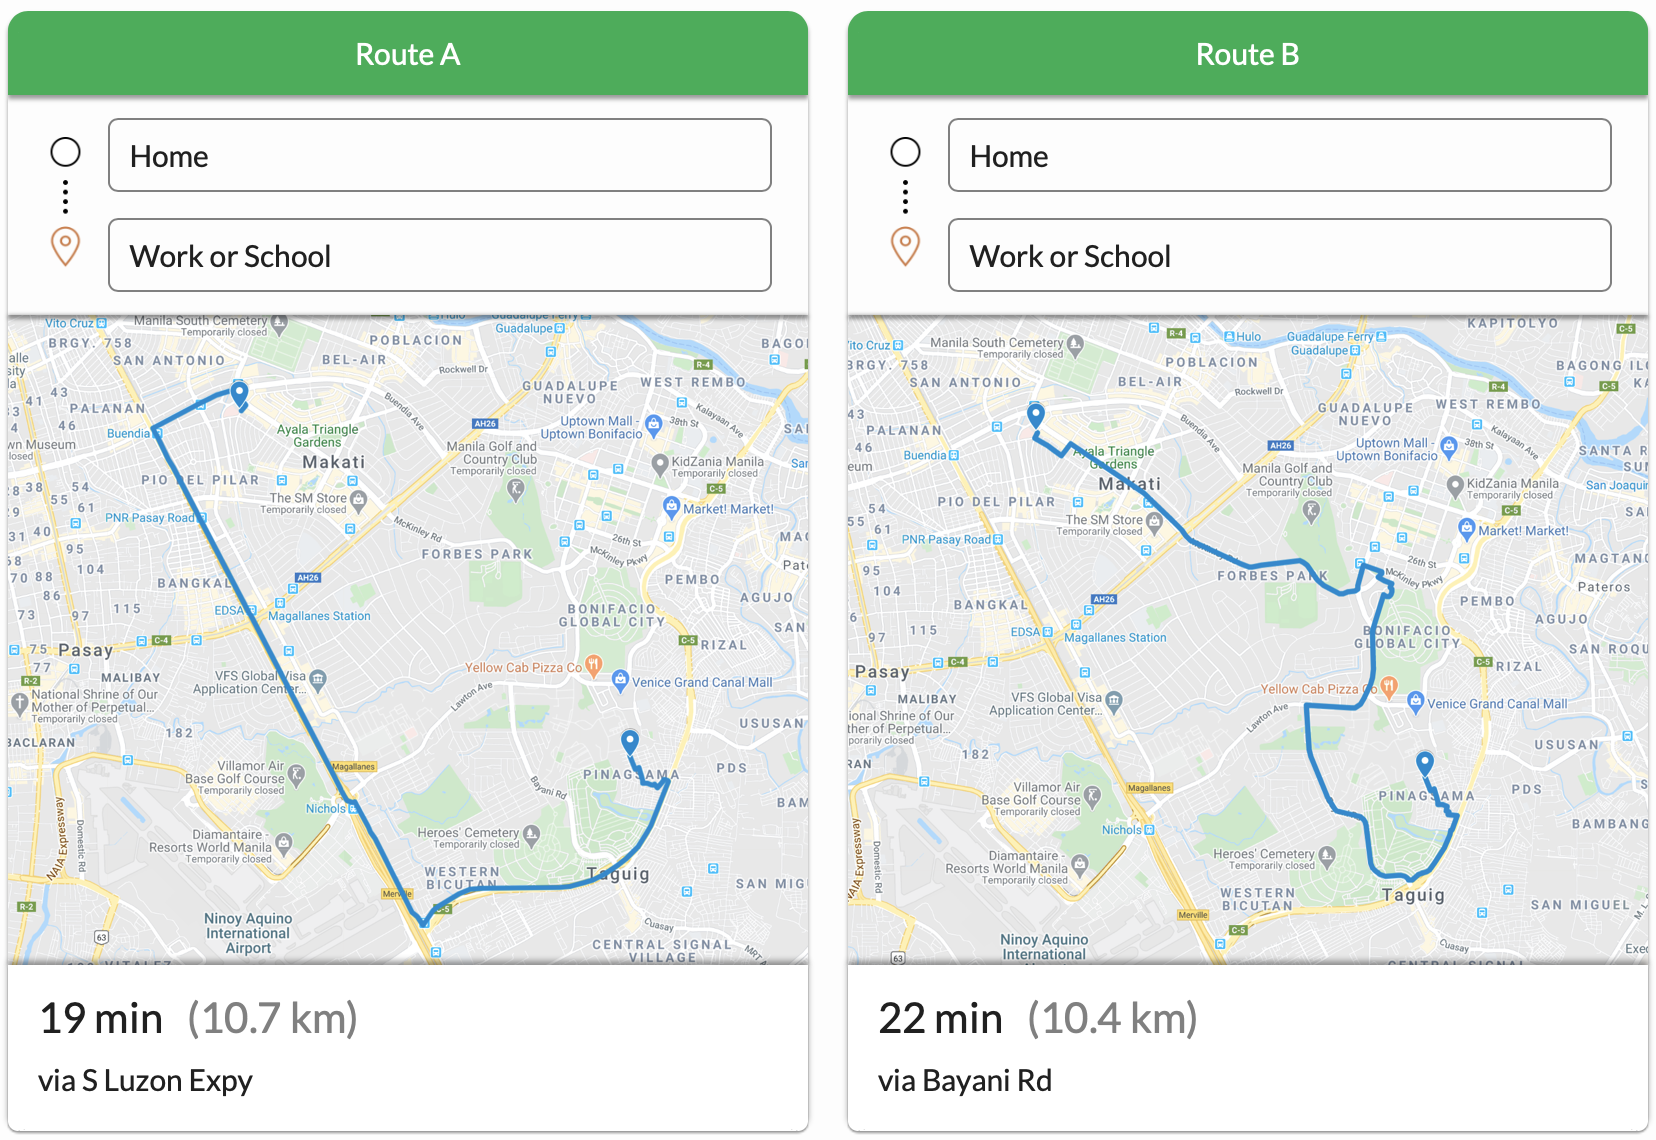
\includegraphics[scale=0.4]{figures/s3-daily-proto.png}
  \caption{The baseline (BL) version of the prototypical navigation app interface. Routes A and B are shown side-by-side. The top part shows the origin and destination with the map below it. The bottom part shows the navigational information that you would typically find in most navigation applications. This part has 27 other versions for each experimental condition.}~\label{fig:s3-daily-proto}
\end{figure}

Before answering the first route choice scenario, participants were asked prepare a timer or clock nearby. For each scenario, they were asked to record the amount of time it took them to make a choice. They were allowed to answer the questionnaire any time within the day but they have to be submitted before the day ends.

\subsubsection{Post-Hoc Questionnaires}
On their last day of the online experiment, they were given two post-hoc questionnaires along with the Day 7 questionnaire. The first questionnaire asks about their demographic and socioeconomic information, and driving experience. The second questionnaire ask them to make pairwise comparisons between the different experimental conditions used in the online experiment.  

\subsubsection{Interviews}
After all 28 participants are completed, we will send invitations for a short interview. I will ask about their qualitative feedback on the sets of motivative and familiarity information shown to them. They will also be presented with their most preferred condition after the pairwise comparison task and asked why they think that is the most convincing combination for them.

\section{Design}
The interface prototype mimics the typical design of most modern navigation applications in the market (e.g. Google Maps, Waze). The screen shows the origin and destination of the trip at the top and a map in the middle. The bottom of the screen shows the navigational information section, for which we created 7 versions. But for all versions of the navigational information section, it always contains the basic set of estimated travel time, total distance and name(s) of major roads. Figure \ref{fig:s3-daily-proto} shows the baseline (BL) version that features the basic set of information. For the six other versions, new information are added on top and bottom parts of the navigational information section. In Figure \ref{fig:s3-navi-parts}, the motivative information is added on the gray box at the top and the familiarity information is added below the name of a major road. Both use the same font size to reduce bias in visual hierarchy. Figure \ref{fig:s3-versions} shows all six versions for each combination.

\begin{figure}[h]
\centering
  
\includegraphics[scale=.8]{figures/s3-navi-parts.png}
  \caption{The additional parts of the navigational information section for the 6 treatment conditions.}~\label{fig:s3-navi-parts}
\end{figure}

\begin{figure}[h]
\centering
  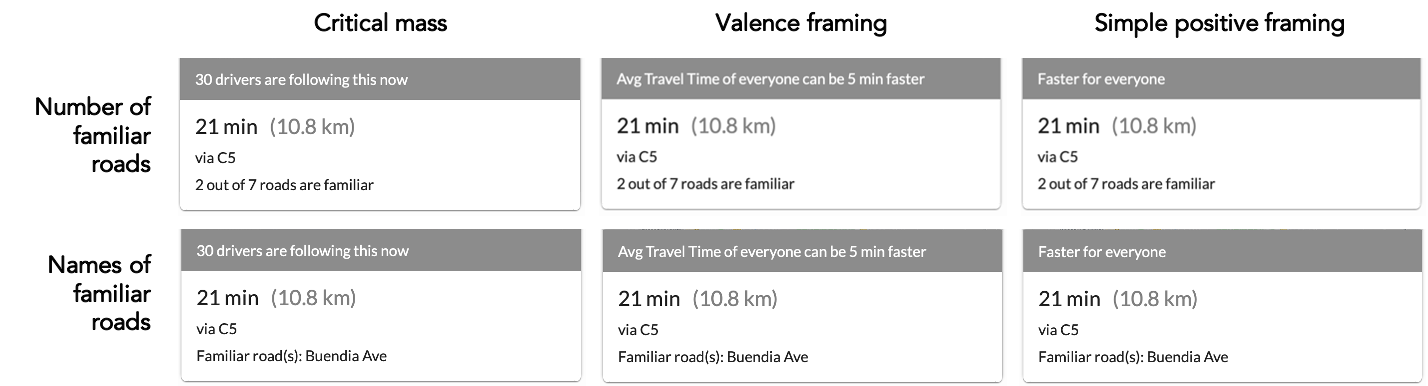
\includegraphics[scale=0.55]{figures/s3-versions.png}
  \caption{The design versions of the navigational information section that adds different combinations of motivative and familiarity information. The versions aligned in the same column use the same motivative information. For example, the two versions in the leftmost column both show critical mass (C) information. The versions in the same row use the same familiarity information.}~\label{fig:s3-versions}
\end{figure}

\section{Materials and Measures}
Because of the remote nature of this study, the participants were asked to answer a number of questionnaires using Google Forms.

\subsection{Measuring Motivation}
We are also interested in understanding whether our autonomy-supportive motivative information are effective in promoting the unselfish route for different regulatory styles and causality orientations. We used two standard questionnaires to measure motivation based on SDT constructs. 

The General Causality Orientation Scale (GCOS)\cite{Deci1985GCOS} measures people's causality orientations on three sub-scales, namely autonomy, control and impersonal. We used the standard 12-item vignette and followed the recommended scales and ordering. Each question presents a scenario with three possible responses. Participants are asked to rate on a scale of 1 to 7 the likelihood that they will respond to the given situation in a certain way. 

On the other hand, the Motivation to Volunteer Scale (MVS)\cite{grano2008motives} measures a person's volunteering motivation based on 24 items. Each of the 6 behavior regulatory styles is represented by 4 items. Participants were asked to what extent do each item correspond to their personal motives for engaging in volunteering. They gave ratings on a scale of 1 (does not correspond at all) to 5 (corresponds exactly). Items were randomized to avoid ordering effect. Because the MVS questionnaire is relatively long, we also added an attention check item. At the end of the preliminary survey, we also asked them about their volunteering experience: ``How often have you participated in volunteering activities in the past three months on average?'' Because the COVID-19 pandemic has unexpectedly motivated people to volunteer, we asked a second question ``How often have you participated in volunteering activities on average from October to December 2019 (before COVID-19 pandemic)?'' for them recall their volunteering frequency before the pandemic and to check for consistency with the first question. Both questions were answered using three options: Never, Once a week and Twice a week or more.

For both GCOS and MVS, we will compute the mean score per sub-scale and use it in the analysis.

\subsection{Route Recommendations}
The route recommendations used in the questionnaires were personalized for each participant using the information they provided from the preliminary survey. For each type of trip, we searched for the fastest route and a sub-optimal route using Google Maps. Searches were done during mid-day to maintain consistency across participants. The fastest route is the route recommendation with the shortest travel time while the sub-optimal route is the recommendation with the longest distance and or longer travel time. The sub-optimal route was used as the unselfish route and assigned as Route B. Route A is always the fastest. To prepare the maps used in the prototypes, we traced the recommended routes using Google My Maps. 

For each participant, a total of 8 route recommendations were prepared. 

\subsubsection{Familiarity Information}
For the daily route choice tasks in this study, the familiarity information was gathered from the preliminary survey where participants are asked to list down all roads that they can possibly recall. 

For the \textit{Name of familiar roads} information, we only showed at most two road names at a time. If the participant is familiar with more than 1 road along the route, we will show the familiar road that is not shown as a major road according to Google Map results. If there is only 1 familiar road and it is the same as the major road(s) returned by Google Maps, then we will just repeat that information.

\subsection{Stated Route Choice}
The daily route choice questionnaires contain 4 binary route choice tasks. They were instructed that they will be making 4 independent trips: 
\begin{itemize}
    \item Work/School to Home
    \item Home to Work/School
    \item Work/School to a frequently visited place
    \item Home to a frequently visited place 
\end{itemize}

Before seeing the prototypes, they were asked to imagine the following scenario:
\begin{quote}
    In each trip, imagine that you are just about to leave and go to a destination. Before leaving your point of origin, you bring out your smartphone and open a navigation application. You are not driving yet. You type your destination in the navigation application and search for routes. Two route suggestions are shown and you have to choose which one to follow. For all route suggestions, you are shown a static map of the route, the estimated travel time, distance and a major road included in the route. Assume that these navigational information are reliable and that you will arrive at your destination on time regardless of choice. 
\end{quote}

Participants were also asked to imagine that a hypothetical Traffic Management System is active during the trips using the following prompt:
\begin{quote}
    Imagine that your city has implemented a Traffic Management System (TMS) to help optimize the traffic flow on its roads. It is run by the city government and receives constant traffic updates in order to make proper traffic assessments. Assume that the information they collect and use are reliable. Its goal is to equally distribute active cars in the road network so that everyone benefits. In order to achieve this, it gives recommendations to connected drivers. However, it does not always distribute drivers to optimize traffic flow. It only happens when they anticipate that many drivers will start using the roads. 

    Your navigation application is connected to this system and it adjusts the route suggestions based on what the TMS recommends. When it predicts that traffic congestion will occur or has already happened, it will now recommend a route that will help ease traffic flow in other areas, along with the usual recommendation of the fastest route. The route suggestions may include 2 types of additional information to help you with your route choice. The first type of information describes how the route can contribute to everyone's travel time. The second information describes how familiar it is to you. You are free to accept or ignore the recommendations and additional information. You will not receive any penalty. 

    In all of the trips, assume that the TMS is detecting traffic congestion on some roads. The traffic flow is now being distributed and you are part of it.
\end{quote}

\subsection{Pairwise Comparison}
On top of recording their stated preferences after seeing different types of navigational information, we also wanted to measure their relative preferences using pairwise comparison. For this, we only used the prototypes for the home-to-work trips. Participants were asked to compare 21 pairs of the 7 design versions. We repeated 1 item to act as attention check and even check for consistency of answers. In total, there were 22 pairwise comparisons made.

\section{Results}
This study is currently ongoing.

For the analysis of route choice task data, I plan to do an ANOVA and or GEE (Generalized Estimating Equations). The objective is to estimate the population average effects and investigate the likelihood that the population will change their route choice behavior given a pair of motivative and familiarity information.

For the analysis of the pairwise comparison data, I plan to construct a  Loglinear Bradley-Terry model. The model can give insights on the likelihoods (worth estimates) that a version is more preferred over another.

I also plan to compare the stated route choices with their pairwise comparisons. I want to investigate whether their relative preferences is conisstent with their route choices. 

Lastly, for both route choice task and pairwise comparison data, I plan to investigate whether they are correlated with the behavior regulatory styles and causality orientations.
